\chapter{Statica del corpo rigido e moti per inerzia}
\section{Statica}

L'obiettivo della statica è trovare le \textbf{configurazioni di equilibrio di un sistema}.
Le configurazioni d'equilibrio sono caratterizzate dalle condizioni
\[
\underline{v}_G = 0,
\qquad
\underline{\omega} = 0,
\qquad
\begin{cases}
\displaystyle \sum_{i=1}^{n} \underline{f}_i^{\mathrm{ext}} = 0, \\[1ex]
\displaystyle \sum_{i=1}^{n} \underline{x}_i \wedge \underline{f}_i^{\mathrm{ext}} = 0.
\end{cases}
\]

\begin{example}{}
Studiamo la statica del seguente sistema

\begin{figure}
\centering
\begin{tikzpicture}[scale=1.15]
  % assi
  \draw[-{Latex[length=3mm]}, line width=0.8pt] (-0.2,-1.0) -- (-0.2,3.5);
  \draw[-{Latex[length=3mm]}, line width=0.8pt] (-0.2,0) -- (5.8,0);

  % punti principali
  \coordinate (A) at (-0.2,2.2);
  \coordinate (O) at (4.8,2.2);
  \coordinate (B) at (4.8,0);
  \coordinate (P) at (-0.2,0);
  \coordinate (G) at (2.3,1.1);

  % segmenti del sistema
  \draw[dashed, line width=0.7pt] (A) -- (O);
  \draw[dashed, line width=0.7pt] (P) -- (O);
  \draw[line width=0.7pt, gray!70!black] (A) -- (B);

  % punti
  \fill (O) circle (1.6pt);
  \fill (B) circle (1.6pt);
  \fill (G) circle (1.6pt);

  % etichette punti
  \node[left] at (A) {$A$};
  \node[above right] at (O) {$0$};
  \node[below right] at (B) {$B$};
  \node[above right] at (G) {$G$};

  % molla
  \draw[orange!90!black, line width=0.9pt]
    (-0.2,2.2) -- (-0.2,2.32)
    -- (-0.30,2.42) -- (-0.10,2.52)
    -- (-0.30,2.62) -- (-0.10,2.72)
    -- (-0.30,2.82) -- (-0.10,2.92)
    -- (-0.30,3.02) -- (-0.10,3.12)
    -- (-0.2,3.22);

  % forza elastica
  \draw[-{Latex[length=2.5mm]}, red, line width=0.9pt] (-0.2,3.22) -- (-0.2,3.47);
  \node[red, right] at (-0.05,3.38) {$k\ell(1-\cos\theta)\,\hat{\jmath}$};

  % psi
  \draw[-{Latex[length=2.5mm]}, blue, line width=0.9pt] (A) -- (1.15,2.2);
  \node[blue, above] at (0.63,2.2) {$\underline{\psi}$};

  % phi
  \draw[-{Latex[length=2.5mm]}, blue, line width=0.9pt] (B) -- (4.8,1.3);
  \node[blue, right] at (4.85,0.78) {$\underline{\varphi}$};

  % peso
  \draw[-{Latex[length=2.5mm]}, red, line width=0.9pt] (G) -- (2.3,-0.82);
  \node[red, below] at (2.3,-0.82) {$mg(-\hat{\jmath})$};

  % angolo theta
  \draw[green!60!black, line width=0.8pt] (-0.2,1.75) arc[start angle=-90,end angle=-24,radius=0.45];
  \node[green!60!black] at (0.18,1.48) {$\theta$};

  % triedro
  \draw[-{Latex[length=2mm]}, purple, line width=0.8pt] (-0.2,0) -- (0.7,0);
  \node[purple, below] at (0.35,0) {$\hat{\imath}$};

  \draw[-{Latex[length=2mm]}, purple, line width=0.8pt] (-0.2,0) -- (-0.2,0.9);
  \node[purple, left] at (-0.2,0.45) {$\hat{\jmath}$};

  \draw[purple, line width=0.8pt] (-1.05,-0.52) circle (0.14);
  \fill[purple] (-1.05,-0.52) circle (0.045);
  \node[purple, below left] at (-0.88,-0.63) {$\hat{k}$};

  % quota l
  \draw[line width=0.8pt] (-1.42,0) -- (-1.42,3.2);
  \draw[line width=0.8pt] (-1.55,0) -- (-1.29,0);
  \draw[line width=0.8pt] (-1.55,3.2) -- (-1.29,3.2);
  \node[left] at (-1.42,1.6) {$\ell$};
\end{tikzpicture}
\end{figure}

Imponiamo i vincoli della statica con polo $\underline{x}_0$ per i momenti
\[
\left\{
\begin{aligned}
\underline{\psi} + k\ell(1-\cos\theta)\,\hat{\jmath} + \underline{\varphi} - mg\,\hat{\jmath} &= 0 \\
(\underline{x}_A-\underline{x}_0)\wedge k\ell(1-\cos\theta)\,\hat{\jmath} + (\underline{x}_G-\underline{x}_0)\wedge -mg\,\hat{\jmath} &= 0
\end{aligned}
\right.
\qquad \Rightarrow \qquad
\]
\[
\Rightarrow
\left\{
\begin{aligned}
\psi &= 0 \\
k\ell(1-\cos\theta)+\varphi-mg &= 0 \\
(-\ell\sin\theta)\,k\ell(1-\cos\theta)\,\hat{k} + \frac{\ell}{2}mg\sin\theta\,\hat{k} &= 0
\end{aligned}
\right.
\]

\[
\Rightarrow
\left\{
\begin{aligned}
\psi &= 0 \\
k\ell(1-\cos\theta)+\varphi-mg &= 0 \\
-k\ell\sin\theta(1-\cos\theta)+\frac{mg}{2}\sin\theta &= 0
\end{aligned}
\right.
\]

Se pongo $\theta=\pi \wedge \theta\neq 0$ allora
\[
-k\ell(1-\cos\theta)+\frac{mg}{2}=0
\;\Rightarrow\;
k\ell\cos\theta=k\ell-\frac{mg}{2}
\;\Rightarrow\;
\cos\theta=1-\frac{mg}{2k\ell}
\]

Dal momento che \qquad $-1<\cos\theta<1$ \qquad allora
\[
-1<1-\frac{mg}{2k\ell}<1
\;\Leftrightarrow\;
-2<-\frac{mg}{2k\ell}<0
\;\Leftrightarrow\;
0<\frac{mg}{2k\ell}<2
\;\Leftrightarrow\;
0<mg<2k\ell
\;\Leftrightarrow\;
\frac{mg}{k\ell}<4
\]

Se $\dfrac{mg}{k\ell}<4$ la condizione \qquad $\cos\theta=1-\dfrac{mg}{2k\ell}$ \qquad dà 2 angoli \qquad $\theta_1,\theta_2$.

Una configurazione di equilibrio si ottiene anche per \qquad $\theta_3=0$ \quad e \quad $\theta_4=\pi$.

Notiamo che $\theta_3,\theta_4$ non sono vincolate a condizioni sui dati del sistema e quindi sono condizioni di equilibrio per ogni istanza del problema.

Notiamo infine che $\psi$ e $\varphi$ sono incognite e sono unicamente determinate da $\theta$.
\end{example}

\section{Moti per inerzia}

La condizione di staticità per il corpo rigido può essere considerata come un caso particolare di moto per inerzia. Diciamo che un corpo rigido si muove per inerzia se sussistono le condizioni
\[
\frac{d}{dt}\, m\underline{v_G} = 0
\qquad
\frac{d}{dt}\left(I_G \underline{\omega}\right) = 0
\]

\begin{example}{}
Consideriamo un sistema formato da un uomo seduto su una sedia che regge una ruota. Ipotizziamo che l'uomo faccia girare la ruota attorno ad un suo asse principale d'inerzia (asse di simmetria) con velocità angolare costante in modulo. Sia $G$ il centro di massa del sistema.

\begin{center}
\begin{tikzpicture}[scale=1.1]
  % asse k uscente/entrante dal foglio
  \draw[red, line width=1pt] (-1.6,2.75) circle (0.24);
  \draw[red, line width=1pt] (-1.73,2.62)--(-1.47,2.88);
  \draw[red, line width=1pt] (-1.73,2.88)--(-1.47,2.62);
  \node[red] at (-1.6,3.12) {$\hat{k}$};

  % assi i e j
  \draw[red, -{Latex[length=3mm]}, line width=1.1pt] (0,2.45)--(0,3.35);
  \node[red] at (0.2,3.15) {$\hat{\imath}$};
  \draw[red, -{Latex[length=3mm]}, line width=1.1pt] (0,2.45)--(1.15,2.45);
  \node[red] at (1.02,2.72) {$\hat{\jmath}$};

  % uomo
  \draw[line width=1.2pt] (0,2.45) circle (0.32);
  \draw[line width=1.2pt] (0,2.13)--(0,0.55);
  \draw[line width=1.2pt] (0,1.52)--(0.62,1.52);
  \draw[line width=1.2pt] (0,0.58)--(0.78,0.82)--(1.02,0.25);
  \draw[line width=1.2pt] (0,0.58)--(0.58,0.48);
  \draw[line width=1.2pt] (-0.15,0.42)--(-0.15,0.18);
  \draw[line width=1.2pt] (-0.15,0.42)--(-0.55,0.42);
  \draw[line width=1.2pt] (-0.55,0.42)--(-0.55,0.22);
  \draw[line width=1.2pt] (-0.55,0.42)--(-0.95,0.42);
  \draw[line width=1.2pt] (-0.95,0.42)--(-0.95,0.22);
  \draw[line width=1.2pt] (-0.78,0.22)--(-0.98,-0.18);
  \draw[line width=1.2pt] (-0.48,0.22)--(-0.25,-0.18);

  % linea verticale arancione, G e mg
  \draw[orange!85!black, {Latex[length=2.5mm]}-{Latex[length=2.5mm]}, line width=1.1pt] (0.62,0.95)--(0.62,2.02);
  \fill[orange!85!black] (0.62,1.50) circle (0.055);
  \node[orange!85!black] at (0.83,1.83) {$G$};
  \node[orange!85!black] at (0.92,0.95) {$mg$};

  % ruota
  \draw[line width=1.2pt] (1.18,1.45) circle (0.35);
  \fill (1.18,1.45) circle (0.05);
  \foreach \a in {0,45,...,315}{
    \draw[line width=1pt] (1.18,1.45)--++(\a:0.3);
  }

  % freccia angolare
  \draw[green!60!black, -{Latex[length=3mm]}, line width=1.1pt]
    (1.78,1.88) arc[start angle=60,end angle=-40,radius=0.58];
  \node[green!60!black] at (2.28,1.95) {$\omega_0$};
\end{tikzpicture}
\end{center}

Dal momento che l'asse di rotazione è un asse principale d'inerzia allora
\[
I_G^{\text{ruota}}\underline{\omega}_0=\omega_0 I_G^{\text{ruota}}\hat{k}=\omega_0 I_G^{\text{ruota},zz}\hat{k}
\]

ovvero il momento angolare ha direzione $\hat{k}$. In particolare, a patto di continuare a effettuare la rotazione attorno ad un asse principale, il momento angolare ha stessa direzione della velocità angolare ad ogni istante $t$, anche se quest'ultima cambia direzione.

L'uomo è inizialmente fermo e quindi $\omega_1=0$ e $I_G^{\text{uomo}}\underline{\omega}_1=0$.

I momenti delle forze esterne al sistema in direzione $\hat{\imath}$ sono nulli e quindi il momento angolare totale in direzione $\hat{\imath}$ deve essere costante ovvero uguale a
\[
\left[\left(I_G^{\text{ruota}}\underline{\omega}_0+I_G^{\text{uomo}}\underline{\omega}_1\right)\cdot\hat{\imath}\right]\hat{\imath}=0
\]

Ad un istante $t>0$ l'uomo inclina la ruota di un angolo $\theta$ facendola girare sempre alla stessa velocità.

\begin{center}
\begin{tikzpicture}[scale=1.15]
  % assi
  \draw[red, -{Latex[length=3mm]}, line width=1.1pt] (0,0)--(0,1.05);
  \node[red] at (0.15,0.9) {$\hat{\imath}$};
  \draw[red, -{Latex[length=3mm]}, line width=1.1pt] (0,0)--(1.0,0);
  \node[red] at (0.88,-0.22) {$\hat{k}$};

  % linea tratteggiata
  \draw[dashed, line width=1pt] (1.6,0)--(6.9,0);

  % ruota iniziale
  \draw[gray!70, line width=1pt, pattern=north east lines, pattern color=gray!70]
    (2.25,-0.48) rectangle (2.55,0.48);
  \draw[green!60!black, -{Latex[length=3mm]}, line width=1.1pt] (2.55,0)--(3.45,0);
  \node[green!60!black] at (3.1,0.28) {$\omega_0$};

  % ruota inclinata
  \begin{scope}[shift={(5.55,0)}, rotate=40]
    \draw[gray!70, line width=1pt, pattern=north east lines, pattern color=gray!70]
      (-0.18,-0.58) rectangle (0.18,0.58);
  \end{scope}

  % nuova velocità angolare
  \draw[green!60!black, -{Latex[length=3mm]}, line width=1.1pt] (5.55,0)--++(40:1.25);
  \node[green!60!black] at (6.35,0.85) {$\omega_0$};

  % angolo theta
  \draw[blue, -{Latex[length=2.5mm]}, line width=1pt] (6.0,0) arc[start angle=0,end angle=40,radius=0.45];
  \node[blue] at (6.28,0.28) {$\theta$};
\end{tikzpicture}
\end{center}

Allora
\[
I_G^{\text{ruota}}\underline{\omega}_0=\omega_0 I_G^{\text{ruota},zz}\cos\theta\,\hat{k}+\omega_0 I_G^{\text{ruota},zz}\sin\theta\,\hat{\imath}
\]

Per quanto detto prima il momento angolare totale lungo $\hat{\imath}$ deve rimanere nullo ovvero
\[
I_G^{\text{ruota},zz}\omega_0\sin\theta+I_G^{\text{uomo},xx}\omega_1=0
\qquad\Rightarrow\qquad
\omega_1=-\frac{I_G^{\text{ruota},zz}\omega_0\sin\theta}{I_G^{\text{uomo},xx}}
\]

L'uomo inizia quindi a girare in senso orario.

\end{example}

\begin{example}{}
Per lo stesso motivo dell'esempio precedente un pattinatore allarga le gambe e braccia per rallentare e le chiude per andare più veloce. Infatti
\[
I_G^1 \omega_1 = I_G^2 \omega_2
\]
con
\[
I_G^1 > I_G^2 \Rightarrow \omega_2 > \omega_1
\]
\end{example}

Analizziamo meglio i vincoli del moto per inerzia.
\[
\frac{d}{dt}\left(m\underline{v}_G\right)=0 \Leftrightarrow m\frac{d}{dt}\underline{v}_G=0
\Rightarrow
\left\{
\begin{aligned}
m\frac{d}{dt}v_G^x &= 0\\
m\frac{d}{dt}v_G^y &= 0\\
m\frac{d}{dt}v_G^z &= 0
\end{aligned}
\right.
\Rightarrow
\left\{
\begin{aligned}
v_G^x &= C_x \in \mathbb{R}\\
v_G^y &= C_y \in \mathbb{R}\\
v_G^z &= C_z \in \mathbb{R}
\end{aligned}
\right.
\Rightarrow
\underline{v}_G(t)=\underline{v}_G(0)\qquad \forall\ t
\]

Lo stesso non si può fare con il secondo infatti
\[
\frac{d}{dt}\left(I_G\omega\right)=0 \not\Rightarrow I_G\frac{d}{dt}(\omega)=0
\]

dal momento che $I_G$ è in realtà una funzione del tempo perché questa dipende dalla distribuzione delle masse dato un orientamento del corpo rigido.

Ad esempio
\[
I_G^{11}=\sum_{i=1}^{n}m_i\left(y_i^2+z_i^2\right)
\]
dipende dall'orientamento del corpo rigido rispetto al sistema di assi coordinati.

La soluzione è quella di usare un sistema di assi coordinati mobili solidali al corpo così che la matrice d'inerzia sia costante.

Al tempo $t=0$ scelgo gli assi $\hat{\imath}(t),\hat{\jmath}(t),\hat{k}(t)$ orientati come gli assi principali d'inerzia. Così possiamo scrivere per ogni istante $t$
\[
I_G=
\begin{pmatrix}
I_G^{xx} & 0 & 0\\
0 & I_G^{yy} & 0\\
0 & 0 & I_G^{zz}
\end{pmatrix}
\qquad
\omega=
\begin{pmatrix}
\omega_x\\
\omega_y\\
\omega_z
\end{pmatrix}
\qquad \Rightarrow \qquad
I_G\omega = I_G^{xx}\omega_x\,\hat{\imath}(t)+I_G^{yy}\omega_y\,\hat{\jmath}(t)+I_G^{zz}\omega_z\,\hat{k}(t)
\]

Prima di andare avanti ci serve la seguente.

\begin{lemma}{}[Formula di Poisson]
Sia $O$ un punto di un corpo rigido e sia $\{O,\underline{e}_1,\underline{e}_2,\underline{e}_3\}$ un qualsiasi riferimento ortonormale solidale al corpo rigido. Allora $\forall i=1,\ldots,3$ vale
\[
\dot{\underline{e}}_i=\underline{\omega}\wedge\underline{e}_i
\]
\end{lemma}
\inizioapprof
\begin{proof}
Consideriamo $\{O,\underline{e}_1,\underline{e}_2,\underline{e}_3\}$ e un punto $P$ del corpo tale che
\[
\underline{x}_P-\underline{x}_O=\underline{e}_i
\]
Allora vale
\[
\underline{v}_P=\underline{v}_O+\underline{\omega}\wedge\underline{e}_i
\qquad\Rightarrow\qquad
\underline{v}_P-\underline{v}_O=\underline{\omega}\wedge\underline{e}_i
\]
Ma
\[
\frac{d}{dt}\,\underline{e}_i=\frac{d}{dt}\left(\underline{x}_P-\underline{x}_O\right)=\underline{v}_P-\underline{v}_O
\]
allora
\[
\dot{\underline{e}}_i=\underline{\omega}\wedge\underline{e}_i \quad \forall i = 1 , \ldots , 3.
\]


\end{proof}
\fineapprof
Riscriviamo il vincolo
\[
\frac{d}{dt}\left(I_G\underline{\omega}\right)=
\frac{d}{dt}\left(I_G^{xx}\omega_x\hat{\imath}(t)+I_G^{yy}\omega_y\hat{\jmath}(t)+I_G^{zz}\omega_z\hat{k}(t)\right)=
\]
\[
= I_G^{xx}\dot{\omega}_x\hat{\imath}
+ I_G^{xx}\omega_x\frac{d\hat{\imath}}{dt}
+ I_G^{yy}\dot{\omega}_y\hat{\jmath}
+ I_G^{yy}\omega_y\frac{d\hat{\jmath}}{dt}
+ I_G^{zz}\dot{\omega}_z\hat{k}
+ I_G^{zz}\omega_z\frac{d\hat{k}}{dt}
=0
\]

Per la formula di Poisson si ha che
\[
\frac{d\hat{\imath}}{dt}=\underline{\omega}\wedge\hat{\imath}
\qquad
\frac{d\hat{\jmath}}{dt}=\underline{\omega}\wedge\hat{\jmath}
\qquad
\frac{d\hat{k}}{dt}=\underline{\omega}\wedge\hat{k}
\]

Semplifichiamo la notazione : \quad $I_G^{xx}=I_1 \qquad I_G^{yy}=I_2 \qquad I_G^{zz}=I_3$

\[
\Rightarrow\quad
I_1\dot{\omega}_x\hat{\imath}
+I_1\omega_x(\underline{\omega}\wedge\hat{\imath})
+I_2\dot{\omega}_y\hat{\jmath}
+I_2\omega_y(\underline{\omega}\wedge\hat{\jmath})
+I_3\dot{\omega}_z\hat{k}
+I_3\omega_y(\underline{\omega}\wedge\hat{k})
=0
\]

e dal momento che
\[
\underline{\omega}\wedge\hat{\imath}
=
\begin{vmatrix}
\hat{\imath} & \hat{\jmath} & \hat{k}\\
\omega_x & \omega_y & \omega_z\\
1 & 0 & 0
\end{vmatrix}
= \omega_z\hat{\jmath}-\omega_y\hat{k}
\qquad
\underline{\omega}\wedge\hat{\jmath}
=
\begin{vmatrix}
\hat{\imath} & \hat{\jmath} & \hat{k}\\
\omega_x & \omega_y & \omega_z\\
0 & 1 & 0
\end{vmatrix}
= -\omega_z\hat{\imath}+\omega_x\hat{k}
\]
\[
\underline{\omega}\wedge\hat{k}
=
\begin{vmatrix}
\hat{\imath} & \hat{\jmath} & \hat{k}\\
\omega_x & \omega_y & \omega_z\\
0 & 0 & 1
\end{vmatrix}
= \omega_y\hat{\imath}-\omega_x\hat{\jmath}
\]

\[
\Rightarrow\quad
I_1\dot{\omega}_x\hat{\imath}
+I_1\omega_x(\omega_z\hat{\jmath}-\omega_y\hat{k})
+I_2\dot{\omega}_y\hat{\jmath}
+I_2\omega_y(-\omega_z\hat{\imath}+\omega_x\hat{k})
+I_3\dot{\omega}_z\hat{k}
+
+I_3\omega_z(\omega_y\hat{\imath}-\omega_x\hat{\jmath})
=0
\]

\[
\Rightarrow
\left\{
\begin{aligned}
I_1\dot{\omega}_x - I_2\omega_y\omega_z + I_3\omega_y\omega_z &= 0\\
I_2\dot{\omega}_y + I_1\omega_x\omega_z - I_3\omega_x\omega_z &= 0\\
I_3\dot{\omega}_z - I_1\omega_x\omega_y + I_2\omega_x\omega_y &= 0
\end{aligned}
\right.
\qquad \Rightarrow \qquad
\left\{
\begin{aligned}
\dot{\omega}_x &= \omega_y\omega_z\,\frac{I_2-I_3}{I_1}\\
\dot{\omega}_y &= \omega_x\omega_z\,\frac{I_3-I_1}{I_2}\\
\dot{\omega}_z &= \omega_x\omega_y\,\frac{I_1-I_2}{I_3}
\end{aligned}
\right.
\]

Abbiamo ottenuto quelle che chiamiamo \textbf{equazioni del moto per inerzia di un corpo rigido}.\\
 Queste sono 3 equazioni differenziali accoppiate che in generale si risolvono numericamente. Il problema si può risolvere analiticamente quando un corpo ha un asse di simmetria, ovvero quando $I_1=I_2=I$. Allora il sistema diventa
\[
\left\{
\begin{aligned}
\dot{\omega}_x &= \omega_0\omega_y\,\frac{I-I_3}{I}\\[4pt]
\dot{\omega}_y &= \omega_0\omega_x\,\frac{I_3-I}{I}\\[4pt]
\dot{\omega}_z &= 0 \qquad \Rightarrow \qquad \omega_z=\omega_0
\end{aligned}
\right.
\]

Vogliamo arrivare ad un'equazione disaccoppiata
\[
\ddot{\omega}_x=\omega_0\dot{\omega}_y\,\frac{I-I_3}{I}
=\omega_0\omega_0\omega_x\,\frac{I_3-I}{I}\cdot\frac{I-I_3}{I}
=-\omega_0^2\left(\frac{I-I_3}{I}\right)^2\omega_x
\]

L'equazione è quella di un oscillatore armonico semplice e posto
\[
\Omega=\omega_0\frac{I-I_3}{I}
\]
ha soluzione
\[
\omega_x(t)=A\cos(\Omega t+\psi)
\qquad \Rightarrow \qquad
\dot{\omega}_y(t)=\omega_0A\cos(\Omega t+\psi)\frac{I_3-I}{I}
\qquad \Rightarrow
\]
\[
\Rightarrow \qquad
\omega_y(t)=A\sin(\Omega t+\psi)\cdot \omega_0\cdot\frac{I_3-I}{I}\cdot\frac{1}{\Omega}
= A\sin(\Omega t+\psi)
\]

ovvero detto $\omega_z=\omega_0$
\[
\left\{
\begin{aligned}
\omega_x &= A\cos(\Omega t+\psi)\\
\omega_y &= A\sin(\Omega t+\psi)
\end{aligned}
\right.
\]

Notiamo che se consideriamo $\{O , \hat{i'} , \hat{j'} , \hat{k'}\}$ sistema di riferimento fisso e accoppiamo le equazioni e le condizioni
\[
\left\{
\begin{aligned}
\dot{\omega}_x &= \omega_y\omega_z\,\frac{I_2-I_3}{I_1} , \quad  \dot{\omega}_y = \omega_x\omega_z\,\frac{I_3-I_1}{I_2}, \quad \dot{\omega}_z = \omega_x\omega_y\,\frac{I_1-I_2}{I_3}\\
& \underline{\omega}(0) = (\omega_{x0} , \omega_{y0} , \omega_{z0}),\\
\hat{\dot{i}} &= \underline{\omega} \wedge \hat{i}, \quad  \hat{\dot{j}} = \underline{\omega} \wedge \hat{j}, \quad  \hat{\dot{k}} = \underline{\omega} \wedge \hat{k}\\
\hat{i} (0) &= i_{x'0} \hat{i'} + i_{y'0} \hat{j'} + i_{z'0} \hat{k'} \\
\hat{j} (0) &= j_{x'0} \hat{i'} + j_{y'0} \hat{j'} + j_{z'0} \hat{k'} \\
\hat{k} (0) &= k_{x'0} \hat{i'} + k_{y'0} \hat{j'} + k_{z'0} \hat{k'}\\
\underline{v}_G(t) &= \underline{v}_G(0) \quad \forall t
\end{aligned}
\right.
\]
otteniamo una descrizione completa del moto.

\subsection{Stabilità del moto per inerzia di un corpo rigido}
Un'altra condizione che rende risolvibile il sistema in modo analitico è la condizione iniziale
\[
\underline{\omega}(0)=(0,0,\omega_0)
\qquad
\text{(oppure } \underline{\omega}(0)=(\omega_0,0,0),\ \underline{\omega}(0)=(0,\omega_0,0)\text{).}
\]
Vogliamo quindi risolvere il problema di Cauchy
\[
\left\{
\begin{aligned}
\dot{\omega}_x &= \omega_y\omega_z\cdot \frac{I_y-I_z}{I_x} \\
\dot{\omega}_y &= \omega_x\omega_z\cdot \frac{I_z-I_x}{I_y} \\
\dot{\omega}_z &= \omega_x\omega_y\cdot \frac{I_x-I_y}{I_z} \\
\underline{\omega}(0) &= (0,0,\omega_0)
\end{aligned}
\right.
\]

Consideriamo la possibile soluzione
\[
\underline{\omega}(t)=(0,0,\omega_0).
\]
Notiamo che soddisfa il problema di Cauchy infatti
\[
\underline{\omega}(0)=(0,0,\omega_0)
\]
\[
\dot{\omega}_x(t)=0=\omega_y(t)\cdot\omega_z(t)\cdot\frac{I_y-I_z}{I_x}
=0\cdot\omega_0\cdot\frac{I_y-I_z}{I_x}=0
\]
\[
\dot{\omega}_y(t)=0=\omega_x(t)\cdot\omega_z(t)\cdot\frac{I_z-I_x}{I_y}
=0\cdot\omega_0\cdot\frac{I_z-I_x}{I_y}=0
\]
\[
\dot{\omega}_z(t)=0=\omega_x(t)\cdot\omega_y(t)\cdot\frac{I_x-I_y}{I_z}
=0\cdot 0\cdot\frac{I_x-I_y}{I_z}=0
\]

Per l'unicità della soluzione di un problema di Cauchy allora
\[
\underline{\omega}(t)=(0,0,\omega_0)
\]
è l'unica possibile soluzione.


Imponendo quindi la velocità angolare iniziale lungo un asse principale d'inerzia si ottiene un moto semplice da descrivere.
Nella realtà imporre questo tipo di condizione è molto difficile. Vogliamo studiare quindi come piccole perturbazioni della condizione iniziale influenzino la soluzione del sistema. Per fare ciò introduciamo in maniera non rigorosa il concetto di stabilità. Ritorneremo su una trattazione di stabilità più rigorosa nelle prossime lezioni.

\begin{definition}{}
Diciamo che $\underline{\omega}^{*}(t)=(0,0,\omega_0)$ è stabile se assegnando condizioni iniziali ``vicine'' a $\underline{\omega}(0)=(0,0,\omega_0)$ otteniamo una soluzione $\underline{\omega}(t)$ ``vicina'' a $\underline{\omega}^{*}(t)$.
\end{definition}

Per studiare se la soluzione è stabile, consideriamo una condizione iniziale perturbata
\[
\underline{\omega}(0)=(\omega_x^0,\omega_y^0,\omega_0)
\qquad \text{con} \qquad
|\omega_y^0|,\,|\omega_x^0| \ll |\omega_0|.
\]

Scriviamo le equazioni per il problema perturbato nei primi istanti del moto. Suppongo che
\[
\left\{
\begin{aligned}
\omega_x(t) &= \omega'_x(t) \\
\omega_y(t) &= \omega'_y(t) \\
\omega_z(t) &= \omega_0 + \omega'_z(t)
\end{aligned}
\right.
\]

Sostituendo nel sistema si ottiene
\[
\left\{
\begin{aligned}
\dot{\omega}'_x &= \omega'_y(\omega_0+\omega'_z)\,\frac{I_y-I_z}{I_x} \\
\dot{\omega}'_y &= (\omega_0+\omega'_z)\omega_x\,\frac{I_z-I_x}{I_y} \\
\dot{\omega}'_z &= \omega'_x\omega'_y\,\frac{I_x-I_y}{I_z}
\end{aligned}
\right.
\]

Dal momento che stiamo supponendo tutte le funzioni continue per un $t$ sufficientemente piccolo possiamo dire che
\[
|\omega'_x(t)| \ll |\omega_0|,
\qquad
|\omega'_y(t)| \ll |\omega_0|
\]
allora trascuriamo i termini che non contengono $\omega_0$
\[
\left\{
\begin{aligned}
\dot{\omega}'_x &= \omega'_y\,\omega_0\,\frac{I_y-I_z}{I_x} \\
\dot{\omega}'_y &= \omega_0\,\omega'_x\,\frac{I_z-I_x}{I_y} \\
\dot{\omega}'_z &= 0
\end{aligned}
\right.
\]


Derivo la prima equazione e sostituisco la seconda
\[
\ddot{\omega}'_x
=
\dot{\omega}'_y\,\omega_0\,\frac{I_y-I_z}{I_x}
=
\omega_0\,\omega'_x\cdot\frac{I_z-I_x}{I_y}\cdot\omega_0\,\frac{I_y-I_z}{I_x}
=
\frac{\omega_0^2}{I_xI_y}(I_z-I_x)(I_y-I_z)\,\omega'_x
\]

Se
\[
a=(I_z-I_x)(I_y-I_z)<0
\]
allora ho l'equazione dell'oscillatore armonico. In questo caso quindi la perturbazione è limitata dai dati iniziali e quindi possiamo dire che $\underline{\omega}(t)$ è stabile.

Se $a>0$ abbiamo una crescita esponenziale nella perturbazione e quindi possiamo dire che $\underline{\omega}(t)$ è instabile.

\begin{itemize}
    \item $a<0$ se $I_z$ è il più piccolo o il più grande tra i momenti d'inerzia.
    \item $a>0$ se $I_z$ è intermedio tra gli altri due.
\end{itemize}


\section{Il problema del gommista}
Supponiamo di avere una ruota vincolata a ruotare attorno ad un asse che non è principale d'inerzia. Denotiamo il versore dell'asse principale d'inerzia con \(\hat{k}'\) e con \(\underline{\omega}\) la velocità angolare della ruota. L'asse di rotazione è fisso e \(\underline{\omega}\) costante, tale che \(\underline{\omega} \wedge \hat{k}' \neq \underline{0}\).\\

\begin{center}
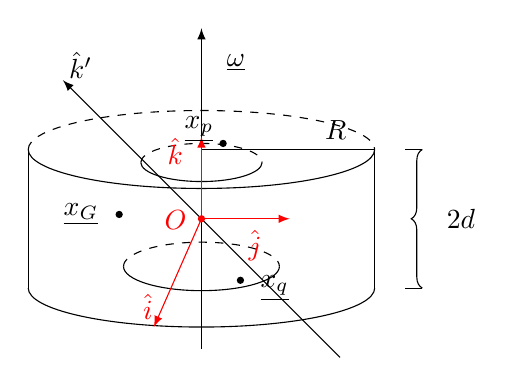
\begin{tikzpicture}[scale=1.1, >=latex]

% cilindro
\draw (-2,0.8) arc[start angle=180,end angle=360,x radius=2,y radius=0.45];
\draw (-2,-0.8) arc[start angle=180,end angle=360,x radius=2,y radius=0.45];
\draw (-2,0.8) -- (-2,-0.8);
\draw (2,0.8) -- (2,-0.8);
\draw[dashed] (-2,0.8) arc[start angle=180,end angle=0,x radius=2,y radius=0.45];

% ellissi interne
\draw (-0.7,0.65) arc[start angle=180,end angle=360,x radius=0.7,y radius=0.22];
\draw[dashed] (-0.7,0.65) arc[start angle=180,end angle=0,x radius=0.7,y radius=0.22];

\draw (-0.9,-0.55) arc[start angle=180,end angle=360,x radius=0.9,y radius=0.28];
\draw[dashed] (-0.9,-0.55) arc[start angle=180,end angle=0,x radius=0.9,y radius=0.28];

% asse verticale e omega
\draw[->] (0,-1.5) -- (0,2.2);
\node[right] at (0.18,1.8) {\(\underline{\omega}\)};

% asse inclinato
\draw[->] (1.6,-1.6) -- (-1.6,1.6);
\node[left] at (-1.15,1.77) {\(\hat{k}'\)};

% raggio orizzontale dell'ellisse esterna superiore
\draw (0,0.8) -- (2,0.8);
\node[above] at (1.55,0.8) {\(R\)};

% sistema di riferimento rosso con origine all'intersezione degli assi
\fill[red] (0,0) circle (1.2pt);
\node[red,left] at (-0.06,-0.02) {\(O\)};

\draw[->,red] (0,0) -- (0,0.95);
\node[red,left] at (-0.1,0.78) {\(\hat{k}\)};

\draw[->,red] (0,0) -- (-0.55,-1.25);
\node[red,left] at (-0.45,-1.02) {\(\hat{i}\)};

\draw[->,red] (0,0) -- (1.02,0);
\node[red,below] at (0.62,-0.02) {\(\hat{j}\)};

% punti e label
\fill (-0.95,0.05) circle (1.2pt);
\node[left] at (-1.08,0.05) {\(\underline{x_G}\)};

\fill (0.25,0.87) circle (1.2pt);
\node[left] at (0.25,1.03) {\(\underline{x_p}\)};

\fill (0.45,-0.71) circle (1.2pt);
\node[right] at (0.57,-0.8) {\(\underline{x_q}\)};

% quota 2d
\draw (2.35,0.8) -- (2.55,0.8);
\draw (2.35,-0.8) -- (2.55,-0.8);
\draw[decorate,decoration={brace,mirror,amplitude=4pt}] (2.55,0.8) -- (2.55,-0.8);
\node[right] at (2.72,0) {\(2d\)};

\end{tikzpicture}
\end{center}

Centriamo un sistema di riferimento \(\{O,\hat{i},\hat{j},\hat{k}\}\) al centro della ruota così che la ruota si estenda lungo \(\hat{k}\) da \(-d\) a \(d\).\\
Supponiamo inoltre che \(\underline{x_G}\) non passi per la direzione di \(\underline{\omega}\) perché la ruota ha subito deformazioni.\\
L'asse fisso impone i vincoli \(\omega_x=\omega_y=0\) a cui corrispondono le reazioni vincolari di momento \(\underline{M}=M_x\hat{\imath}+M_y\hat{\jmath}\). L'idea è che se la ruota è vincolata a ruotare attorno ad un asse che non è principale d'inerzia il momento angolare deve necessariamente variare nel tempo per permettere la rotazione. Abbiamo visto nella scorsa lezione infatti che l'unico modo per cui questo non accada è che l'asse sia principale d'inerzia. Impostiamo la seconda legge cardinale

\[
\frac{d}{dt}\left(I_G\underline{\omega}\right)=\underline{M}
\;\Rightarrow\;
\frac{d}{dt}\left[
\begin{pmatrix}
I_{xx} & I_{xy} & I_{xz} \\
I_{yx} & I_{yy} & I_{yz} \\
I_{zx} & I_{zy} & I_{zz}
\end{pmatrix}
\begin{pmatrix}
0 \\
0 \\
\omega
\end{pmatrix}
\right]
=
\begin{pmatrix}
M_x \\
M_y \\
0
\end{pmatrix}
\;\Rightarrow
\]

\[
\Rightarrow
\begin{cases}
\dfrac{d}{dt}\left(I_{xz}\,\omega\right)=M_x \\[1ex]
\dfrac{d}{dt}\left(I_{yz}\,\omega\right)=M_y
\end{cases}
\]
Qui quello che varia sono proprio $I_{xz}, I_{yz}$ perché il corpo gira attorno ad un sistema di assi non solidali e rispetto al quale non è simmetrico. Vogliamo quindi spostare gli assi principali d'inerzia così che quei momenti d'inerzia siano costanti e uguali a 0.\\
Per fare ciò il gommista deve aggiungere delle masse sul cerchione in modo tale che

\begin{itemize}
\item \(I_{xz}=I_{yz}=0\)
\item \(x_G=y_G=0\)
\end{itemize}

così che \(\hat{k}\) diventi asse principale d'inerzia e che \(M_x=M_y=0\).

Ricordiamo che
\[
I_{xz}=-\sum_i m_i\,x_i\,z_i
\]

\[
I_{yz}=-\sum_i m_i\,y_i\,z_i
\]


Per allineare l'asse principale d'inerzia con \(\underline{\omega}\) sommiamo al sistema 2 masse \(m_p,m_q\) di posizione \(\underline{x_q},\underline{x_p}\).

Per ragioni fisiche vogliamo mettere una massa sul bordo del cerchione superiore e una sul bordo del cerchione inferiore.

\begin{center}
\begin{minipage}{0.45\textwidth}
\centering
\begin{tikzpicture}[scale=1.1,>=latex]
\draw (0,0) circle (2.1);
\draw (0,0) circle (0.95);

\fill (0,0) circle (1.3pt);
\coordinate (P) at ({0.95*cos(50)},{0.95*sin(50)});
\fill (P) circle (1.3pt);

\draw (0,0) -- (P);
\draw[dashed] (0,0) -- (2.1,0);

\draw (0.45,0) arc[start angle=0,end angle=50,radius=0.45];

\node at (0.1,0.45) {\(r\)};
\node at (0.52,0.24) {\(\theta\)};
\node at (1.35,-0.22) {\(R\)};
\node at ($(P)+(0.1,0.28)$) {\(\underline{x_p}\)};

\node at (0,-2.45) {Vista dall'alto};
\end{tikzpicture}
\end{minipage}
\hfill
\begin{minipage}{0.45\textwidth}
\centering
\begin{tikzpicture}[scale=1.1,>=latex]
\draw (0,0) circle (2.1);
\draw (0,0) circle (0.95);

\fill (0,0) circle (1.3pt);
\coordinate (Q) at ({0.95*cos(50)},{0.95*sin(50)});
\fill (Q) circle (1.3pt);

\draw (0,0) -- (Q);
\draw[dashed] (0,0) -- (2.1,0);

\draw (0.45,0) arc[start angle=0,end angle=50,radius=0.45];

\node at (0.1,0.45) {\(r\)};
\node at (0.52,0.24) {\(\psi\)};
\node at (1.35,-0.22) {\(R\)};
\node at ($(Q)+(0.1,0.28)$) {\(\underline{x_q}\)};

\node at (0,-2.45) {Vista dal basso};
\end{tikzpicture}
\end{minipage}
\end{center}
Impongo quindi \(\underline{x_p}=(r\cos\theta,r\sin\theta,d)\), \(\underline{x_q}=(r\cos\varphi,r\sin\varphi,-d)\).

Scriviamo nel caso generale le condizioni

\[
\text{1) il centro di massa è sull'asse } \hat{k}
\]

\[
\text{2) } \hat{k} \text{ asse principale d'inerzia}
\]

\[
\left\{
\begin{aligned}
m\,x_G + m_p\,x_p + m_q\,x_q &= 0\\
m\,y_G + m_p\,y_p + m_q\,y_q &= 0\\
I_{xz} - m_p\,x_p\,z_p - m_q\,x_q\,z_q &= 0\\
I_{yz} - m_p\,y_p\,z_p - m_q\,y_q\,z_q &= 0
\end{aligned}
\right.
\]

Il sistema è nelle 8 incognite \(m_p,m_q,x_p,x_q,y_p,y_q,z_p,z_q\).
Applicando la restrizione per \(\underline{x_p}\) e \(\underline{x_q}\) possiamo ridurre le incognite alle 4 \(\theta,\varphi,m_p,m_q\).

\[
\left\{
\begin{aligned}
m_p\,r\cos\theta + m_q\,r\cos\varphi &= -m\,x_G \qquad \text{(I)}\\
m_p\,r\sin\theta + m_q\,r\sin\varphi &= -m\,y_G \qquad \text{(II)}\\
m_p\,d r\cos\theta - m_q\,d r\cos\varphi &= I_{xz} \qquad \text{(III)}\\
m_p\,d r\sin\theta - m_q\,d r\sin\varphi &= I_{yz} \qquad \text{(IV)}
\end{aligned}
\right.
\]

La soluzione è

\[
m_p=\frac{1}{2r}\sqrt{\left(-m x_G+\frac{I_{xz}}{d}\right)^2+\left(-m y_G+\frac{I_{yz}}{d}\right)^2}
\]

\[
m_q=\frac{1}{2r}\sqrt{\left(-m x_G-\frac{I_{xz}}{d}\right)^2+\left(-m y_G-\frac{I_{yz}}{d}\right)^2}
\]

\[
\theta=\operatorname{atan2}\left(-m y_G+\frac{I_{yz}}{d},-m x_G+\frac{I_{xz}}{d}\right)
\]

\[
\varphi=\operatorname{atan2}\left(-m y_G-\frac{I_{yz}}{d},-m x_G-\frac{I_{xz}}{d}\right)
\]
